
\section{Materiais e Métodos} \label{sec:metodo}

Nesta seção, detalham-se os procedimentos e ferramentas utilizados para a obtenção e análise inicial dos dados que fundamentam este estudo.

\subsection{Descrição do Dataset e Coleta de Dados} \label{subsec:dataset}
A base de dados selecionada para este trabalho consiste em eventos de execução em sandbox (análise dinâmica), especificamente o dataset público disponibilizado por \cite{sgandurra2016}. Esta escolha justifica-se pelo fato de o dataset ser bem referenciado em estudos de segurança e inteligência artificial, servindo como base consolidada para a análise de comportamentos maliciosos \cite{caio2022}.

\subsubsection{A. Natureza e Origem dos Dados} \label{subsubsec:dataset-natureza}
Os dados foram gerados por meio da execução de amostras em um ambiente controlado utilizando a ferramenta \textit{Cuckoo Sandbox} \cite{cuckoosandbox}. Ao contrário da análise estática, a análise dinâmica permite capturar o comportamento real do código em execução, mitigando técnicas de evasão como ofuscação e criptografia de binários \cite{sgandurra2016}. O dataset é composto por um total de 1.524 amostras, divididas em:
\begin{itemize}
    \item \textbf{582 malwares (Ransomware):} Representando 38,19\% do total.
    \item \textbf{942 goodwares (Aplicações legítimas):} Representando 61,81\% do total.
\end{itemize}

As amostras de ransomware estão subdivididas em 11 famílias distintas, permitindo uma análise granular dos diferentes padrões de ataque \cite{sgandurra2016}. Entre as famílias presentes, destacam-se \textit{CryptLocker} (107 amostras), \textit{Locker} (97) e \textit{Reveton} (90), como é listado mais detalhadamente na tabela ~\ref{tab:dataset-stats}.

\subsubsection{B. Variáveis e Engenharia de Atributos (Features)} \label{subsubsec:dataset-variaveis}
O dataset original contém 30.967 atributos binários, que representam a presença (1) ou ausência (0) de uma determinada ação ou evento durante a execução\cite{sgandurra2016}.
Para este estudo foi incialmente desenvolvido um script em python (Figura ~\ref{fig:cod-dataset-stats}) para o levantamento estatístico inicial do dataset (mais detalhado na Tabela ~\ref{tab:dataset-stats}). Estes atributos estão organizados em sete categorias de comportamento:
\begin{itemize}
    \item \textbf{API:} Invocações de chamadas de sistema (\textit{API calls}).
    \item \textbf{DROP:} Extensões de arquivos criados (\textit{dropped}) durante a execução.
    \item \textbf{REG:} Operações em chaves de registro do Windows.
    \item \textbf{FILES:} Operações gerais de sistema de arquivos (leitura, escrita, deleção).
    \item \textbf{FILES\_EXT (EXT):} Extensões dos arquivos envolvidos nas operações de arquivo.
    \item \textbf{DIR:} Operações em diretórios (criação, enumeração).
    \item \textbf{STR:} Strings incorporadas no binário original.
\end{itemize}

\subsection{Estatísticas do Dataset} \label{subsec:dataset-stats}
A Tabela \ref{tab:dataset-stats} apresenta a distribuição detalhada das amostras de ransomware por família, conforme extraído do processamento dos dados brutos.
\begin{figure}[htbp]
	\centering
	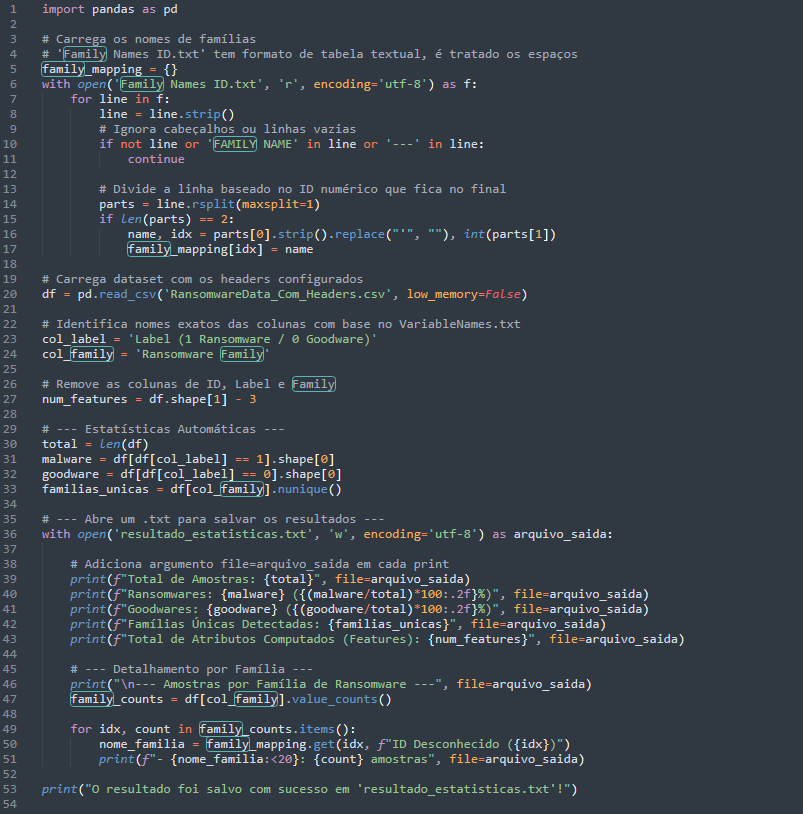
\includegraphics[width=.8\textwidth]{images/codigo_estatistica.png}
	\caption{Script Python para levantamento estatístico do dataset.}
	\label{fig:cod-dataset-stats}
\end{figure}

\begin{table}[htbp]
    \centering
    \caption{Visão Geral e Distribuição de Amostras do Dataset Sgandurra (2016).}
    \label{tab:dataset-stats}
    \begin{tabular}{|l|c|}
    \hline
    \textbf{Métrica} & \textbf{Valor / Quantidade} \\ \hline
    Total de Amostras & 1.524 \\ \hline
    Ransomwares & 582 (38.19\%) \\ \hline
    Goodwares & 942 (61.81\%) \\ \hline
    Famílias Únicas Detectadas & 11 \\ \hline
    Total de Atributos Computados (Features) & 30.967 \\ \hline
    \hline
    \multicolumn{2}{|c|}{\textbf{Amostras por Família de Ransomware}} \\ \hline
    Goodware & 942 \\ \hline
    CryptLocker & 107 \\ \hline
    Locker & 97 \\ \hline
    Reveton & 90 \\ \hline
    Kovter & 64 \\ \hline
    MATSNU & 59 \\ \hline
    Critroni & 50 \\ \hline
    CryptoWall & 46 \\ \hline
    Trojan-Ransom & 34 \\ \hline
    KOLLAH & 25 \\ \hline
    TeslaCrypt & 6 \\ \hline
    PGPCODER & 4 \\ \hline
    \end{tabular}
\end{table}

%\begin{minted}{python}
%def ola_mundo():
%    print("Olá, LaTeX!")
%\end{minted}